\documentclass[fleqn]{hermans-hw}

%\usepackage{haldefs}
\usepackage{amsmath}
\usepackage{float}
\usepackage{notes}
\usepackage{url}
\usepackage{graphicx}
\newcommand{\floor}[1]{\lfloor #1 \rfloor}
\title{Project 1: Search in Pacman}
\duedate{}
\class{CS6300: Artificial Intelligence, Spring 2018}
\institute{University of Utah}
\author{Jake Pitkin}
% IF YOU'RE USING THIS .TEX FILE AS A TEMPLATE, PLEASE REPLACE
% The author WITH YOUR NAME AND UID.
% Replace the due date with anyone you worked with i.e. "Worked with: John McCarthy, Watson, & Hal-9000"

\begin{document}

\maketitle
\section{Depth First Search}
\begin{enumerate}
	\item Is the exploration order what you would have expected? Does Pacman actually go to all the explored squares on his way to the goal?
	
	The exploration order is what I would have expected. As we can see in Figure 1 (where Pacman starts in the bottom right corner) that he doesn't explore spaces close to the start location. Instead he goes for depth before breadth. 
	
	All the explored spaces are not explored. The many dead ends along the way to his goal are expanded by DFS, but are not part of the final path that he travels to the goal.
	
	\begin{figure}[H]
  \centerline{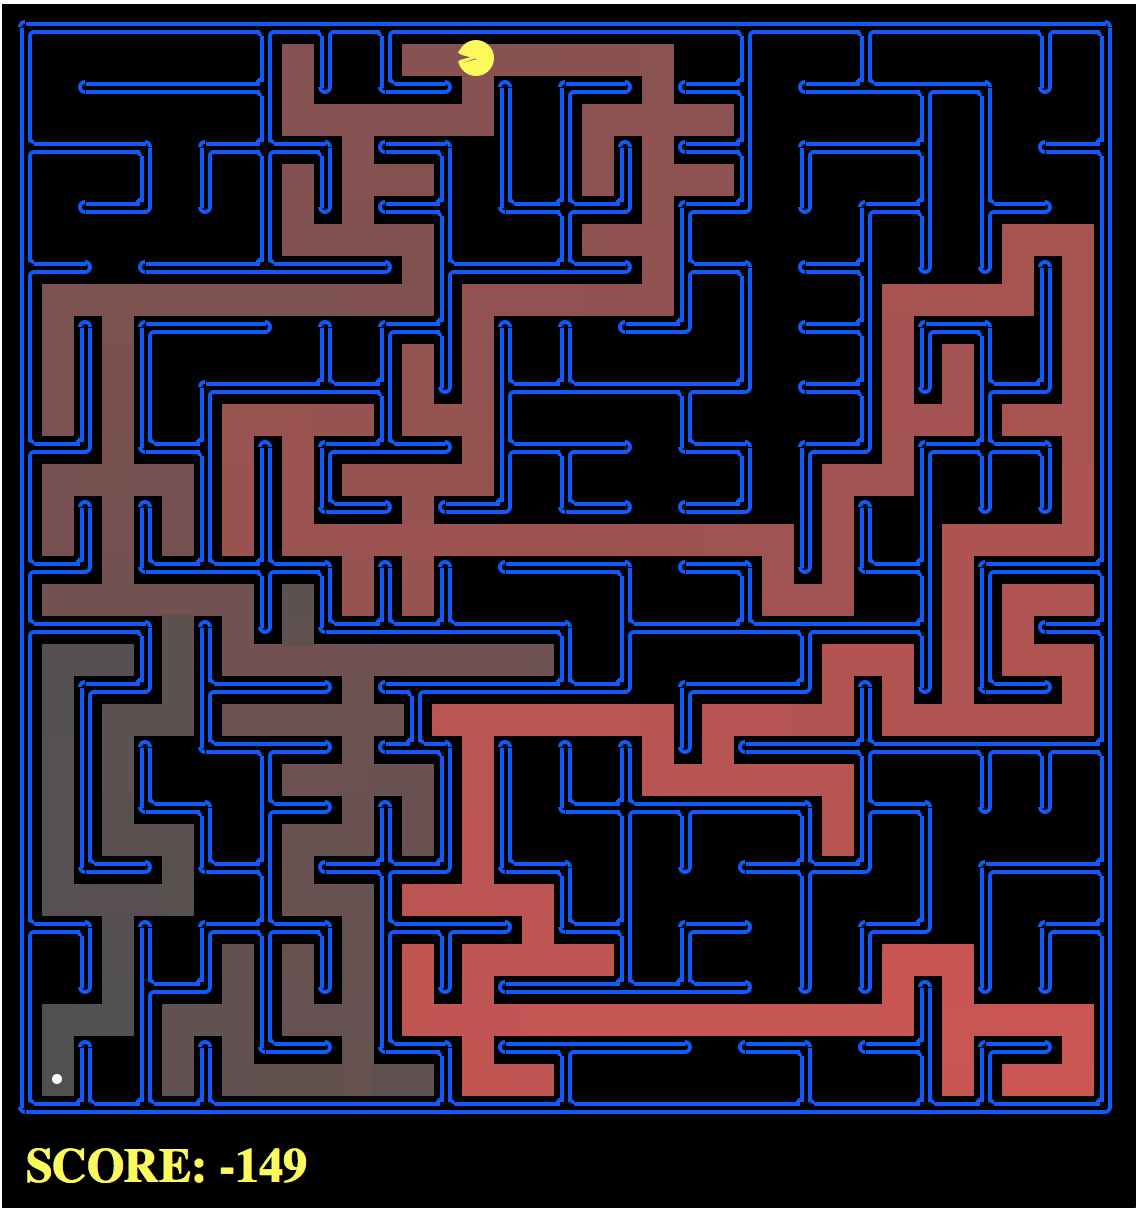
\includegraphics[width=0.5\linewidth]{img_1.png}}
  \caption{Example of DFS on bigMaze.}
\end{figure}
	
	\item Is this a least cost solution? If not, think about what depth-first search is doing wrong.
	
	This is not a least cost solution. One key observation is that during DFS we take the first action and continue until we arrive in a state where all the actions are visited nodes (dead ends). But compared to BFS that considers all actions from the current state instead. The behavior of DFS taking the first action will tend towards longer paths.
\end{enumerate}

\section{Breadth First Search}
\begin{enumerate}
	\item Does BFS find a least cost solution? If so explain why.
	
	In general, BFS does not find a least cost solution in a weighted graph, it finds the shortest path.
	
	But, in the Pacman case were each action has a cost of 1, BFS will find a least cost solution. This is because the shortest path (which it finds) will also be a least cost solution as each action costs 1.
\end{enumerate}

\section{Uniform Cost Search}
\begin{enumerate}
	\item Specify the data structure used from the util.py for the uniform cost search.
	
	To implement uniform cost search, a PriorityQueue data structure was used from util.py. This is needed as we want to select the cheapest node from the frontier at each iteration. As opposed to using the order nodes were queued as in BFS or DFS. 
	
\end{enumerate}

\section{A* Search}
\begin{enumerate}
	\item What happens on openMaze for the various search strategies? Describe your answer in terms of the solution you get for A* and uniform cost search.
	
	On openMaze A* search finds a path of length 54 with 535 search nodes expanded. Compared to uniform cost search which also finds a path of length 54 but expands 682 nodes. Both search algorithms find the same length paths, but A* search does so by expanded less nodes.
	
	In openMaze Pacman starts in the top right corner and the goal is in the bottom left corner and there are very few walls. Uniform search expands the entire maze as can be seen in Figure 2.
	
	In Figure 3, we can see the Manhattan distance heuristic "pull" pacman to the left and avoid a large section of the bottom right of the map.
	
		\begin{figure}[H]
  \centerline{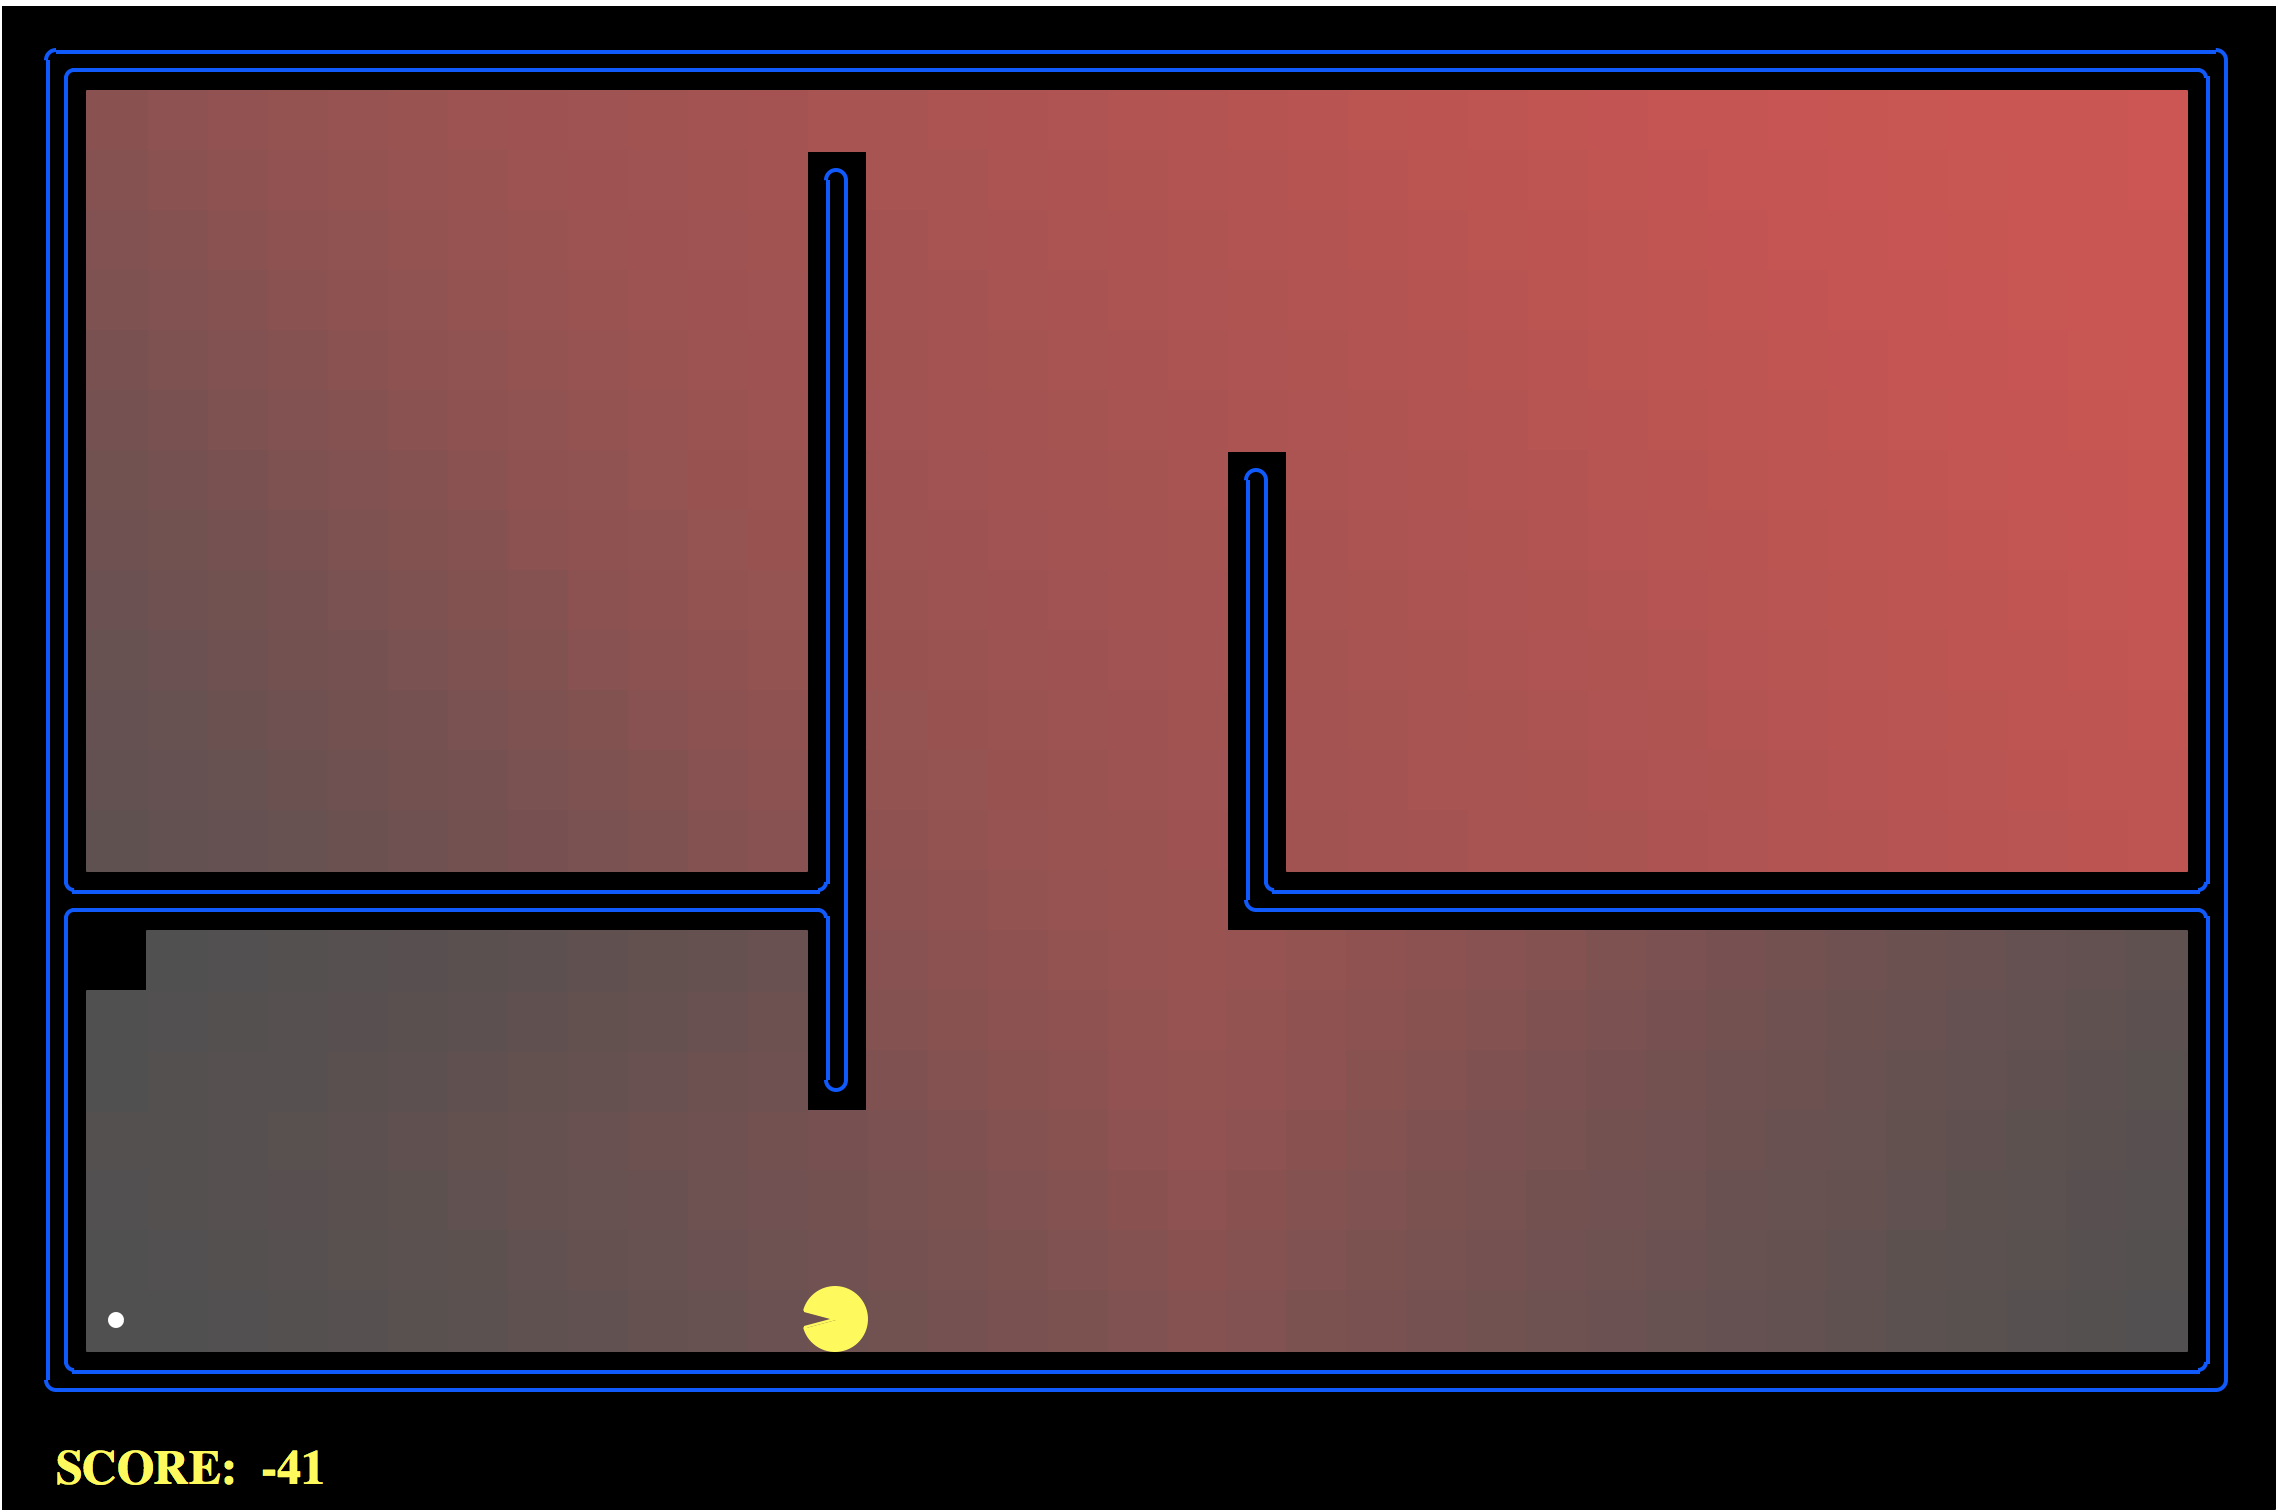
\includegraphics[width=0.5\linewidth]{img_3.png}}
  \caption{Uniform cost search on bigMaze.}
\end{figure}

	\begin{figure}[H]
  \centerline{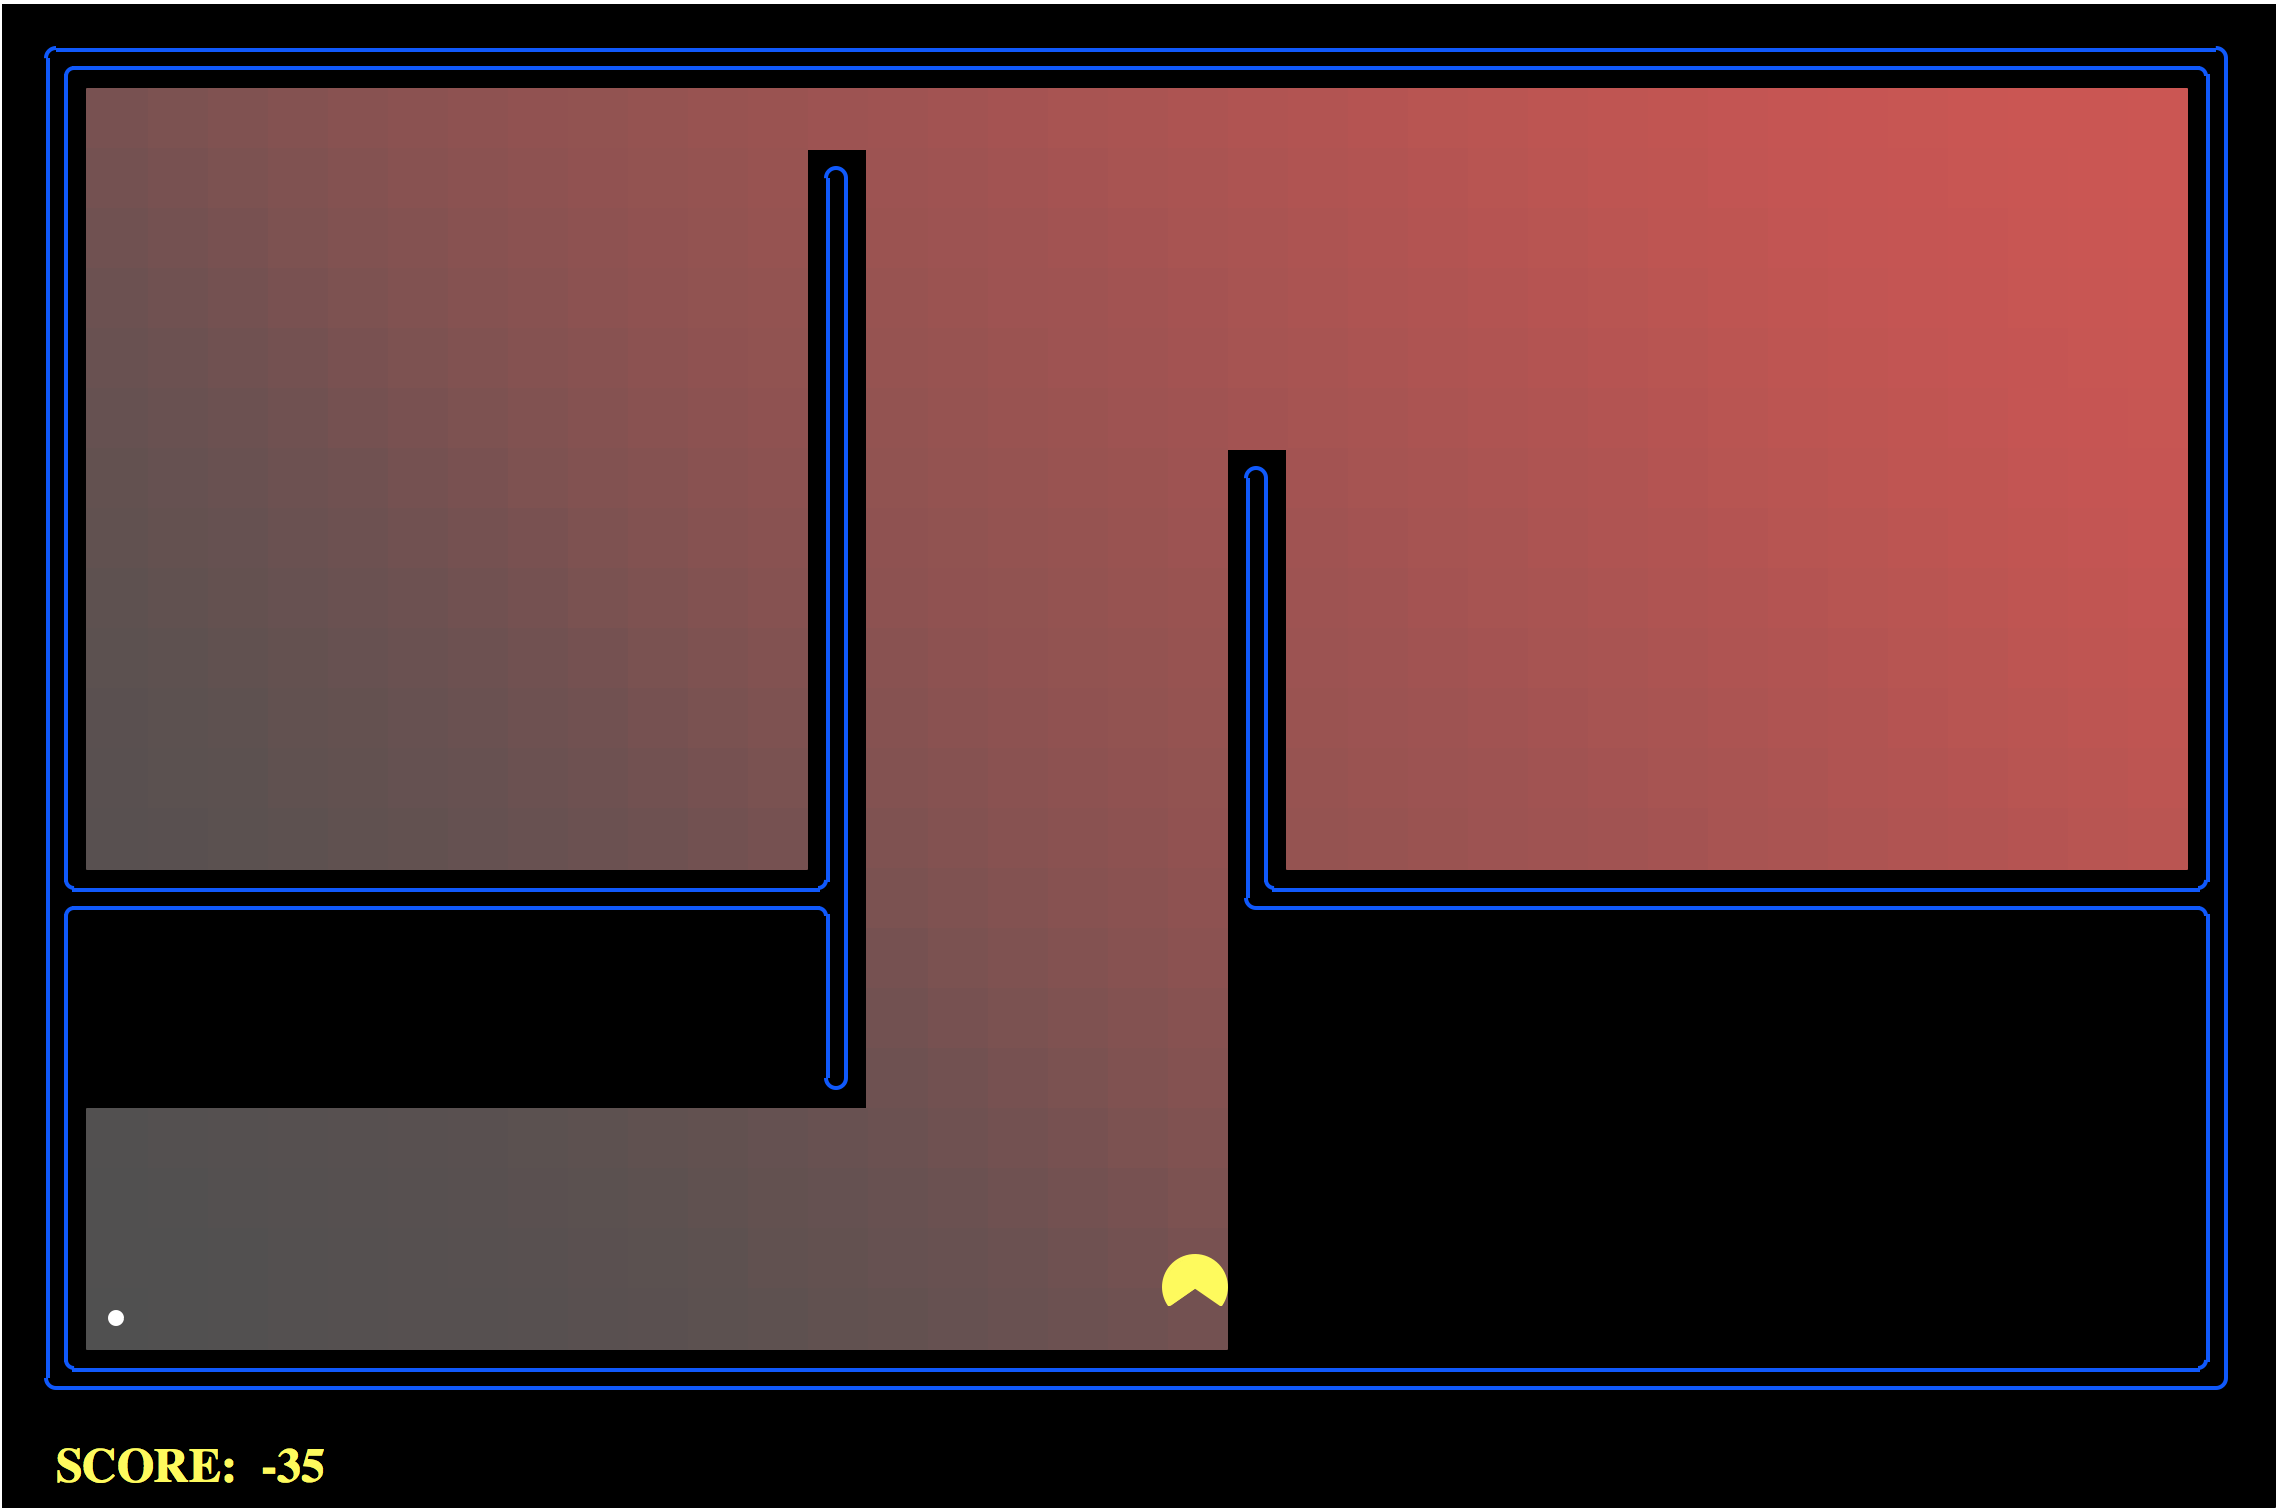
\includegraphics[width=0.5\linewidth]{img_2.png}}
  \caption{A* search on bigMaze.}
\end{figure}
	
\end{enumerate}

\section{Finding All the Corners}
\begin{enumerate}
	\item Describe in a few words the state representation you chose or how you solved the problem of finding all the corners.
	
	I solved the problem of finding all the corners using the following state: the current location and the location of the corners that have yet to be reached. The goal state was defined as a state having traversed all four of the corners.
	
	When using A* search, I used the Manhattan distances to the corners as a heuristic. For each corner that had yet to be traversed, I calculated the Manhattan distance between it and the current location. The shortest Manhattan distance was selected as the heuristic value. If all the corners had been discovered, zero was returned.
\end{enumerate}

\section{Eating All Dots}
\begin{enumerate}
	\item Describe the heuristic you had used for the FoodSearchProblem.
	
	Similar to the corners problem, I used the Manhattan distance as a heuristic. For each dot still uneaten on the map, I calculated the Manhattan distance between it and the current location. The shortest Manhattan distance was selected as the heuristic value. If all the dots had been eaten, zero was returned.
\end{enumerate}

\newpage
\section{Suboptimal Search}
\begin{enumerate}
	\item Explain why the ClosestDotSearchAgent won't always find the shortest possible path through the maze.
	
	Consider an adversarial situation where Pacman will have to perform a lot of backtracking:
	
	XXXXXXXXXXXXXXXXXXXXXXXXXXXXXXXXXXXXXXXXXX \\
	X ($<$ $* \ * \ * \ * \ * \ * \ * \ * \ * \ * \ * \ * \ * \ * \ * \ * \ * \ * \ * \ * \ * \ * \ * \ * \ * \ * \ * \ * \ * \ * \ * \ * \ * \ $X \\
	X$\ \ \ \ $XXXXXXXXXXXXXXXXXXXXXXXXXXXXXXXXXXXXXXX \\
	X $\ \ $ X \\
	X $*$ X \\
	XXXX
	
	That is, there is a long trail of dots one space away from Pacman and a single dot two spaces away from Pacman. He will take the long path of dots under the ClosestDotSearchAgent then backtrack to get the final dot. He could cut his path roughly in half by first grabbing the close dot then taking the long trail.
	
	This is an adversarial situation but similar problems could arise in larger mazes.
	\end{enumerate}

\section{Self Analysis}
\begin{enumerate}
	\item What was the hardest part of the assignment for you?
	
	The hardest part of this assignment for me was coming up with creative heuristics. I am new to the idea of heuristics and it seems to take some practice to scheme up how to apply knowledge about the problem into a heuristic.
	
	\item What was the easiest part of the assignment for you?
	
	The easiest part of the assignment for me was coding up the search algorithms. I have some experience with Python and had seen all the search algorithms in prior courses. Once I understood the supplied framework the work came at a nice pace.
	
	\item What problem(s) helped further your understanding of the course material?
	
	All of them really. The unit tests provided are really well done and the visual representations of the problems provided helped a lot. By implementing the search algorithms I got a deeper understanding of what makes each of the unique and how they are similar. 
	
	\item Did you feel any problems were tedious and not helpful to your understanding of the material?
	
	I didn't find anything tedious about this project. Most of the tedious coding is provided for us; allowing us to focus on the search algorithms themselves and designing heuristics.
	
	\item What other feedback do you have about this homework?
	
	No strong feedback, but I find creating heuristics to be tough. I understand trivial ones such as Manhattan distance, but I had a hard time coming up with anything more creative.
\end{enumerate}

\end{document}
